\chapter{Subjective Experiment}

%- Why do we need ground truth data
%- introduce datasets
%- what is a subjective experiment?
%- Conduct subjective experiment to collect ground truth data

\label{chap:subjective}
This chapter contains the process of designing and conducting our subjective experiment. In Section \ref{sec:groundTruth} we explain how and why collecting ground truth data is important in this project. The next Section \ref{sec:SubjectiveAspects} addresses important aspects when creating a subjective experiment. These sections are followed by the introduction of datasets used in the experiment and application (Section \ref{sec:datasets}) as well as an in-depth description of our subjective experiment in Section \ref{sec:OurSubjectiveExperiment}. At the end of this chapter we introduce the creation of our own dataset in Section \ref{sec:ownData} followed by the evaluation of this dataset in Section \ref{sec:secondse}.

\section{Why Collect Ground Truth Data?}
\label{sec:groundTruth}
Ground truth data is data based on human assessments. The ground truth data is collected by arranging subjective experiments, where human observers are asked to evaluate a set of images according to given criteria \cite{Xphdthesis}. In this project, observers graded facial images. Gathering ground truth data is an essential part of our work, because subjective data is needed to evaluate the performance of the objective assessments. Validation between subjective and objective assessments secure that the FIQMs correspond with how human observers rate facial images. 

\section{Subjective Experiment Aspects}
\label{sec:SubjectiveAspects}
As mentioned in Section \ref{section:academic background}, our lack of experience indicated that an introduction to subjective experiments was needed. The research about this topic made us realize the importance and difficulties with this task. There were several assessments to perform in terms of creating a comprehensive subjective experiments such as type of psychophysical experiment, duration of experiment and observer types.

\subsection{Experiment Method}
There were several psychophysical experiment methods to choose. We based our choice with the method that fitted our experiment the best. The options were between category judgment and rank order. Category judgment is a method where the observers rate facial images based on given criteria. These images are allocated to a category \cite{Xphdthesis}. In rank order the observers are shown multiple images simultaneously and asked to rank them based on given criteria. 

\subsection{Experiment Duration}
The experiment duration is an important factor when conducting a subjective experiment. At one hand, it is essential to give the observers a high number of facial images to grade for the data collecting purposes. At the other hand, having a too long duration of the experiment can cause observer fatigue such as eye fatigue or headache. These kinds of disorders will affect the subjective data negatively.  

\subsection{Types of Observers}
The subjective experiment was available for everyone to perform, but we invited a specific target group that works in this field. The types of participants are divided in two groups: experts and non-experts.

\subsubsection*{Experts}
The experts are the people who were specially invited to complete the experiment. These observers work either for Mobai with facial recognition systems or at NTNU in the Faculty of Information Technology and Electronics. A point of having experts in the field doing the subjective experiment was to quality assure our creation since they to a larger degree can distinguish between quality issues. In addition to that, we were to compare the results between the two groups. 

\subsubsection*{Non-experts}
Non-experts were people with no experience in the biometric field. They were our friends and family of different ages and educations.

\section{Datasets}
\label{sec:datasets}
The usage of facial images in the application and subjective experiment raised GDPR issues. It would strike against the rules if we photographed people on the streets or collected random images on the web without consent from the subjects. The ground truth data in this project was collected on three different data sets provided by Mobai. Table \ref{table:DatasetInformation} displays all datasets used in the project. Combined passport alike was a high resolution dataset with images from the Tufts Face Database \cite{Tufts-Face-Database} and FEI Face Database \cite{FEI-Face-Database}, which has a similarity to passport or id photos, hence the title. The set consisted of 98 facial images of people with different poses, facial expressions and lighting. All images were taken using a Nikon D3100 with a dark blue or light grey background, as depicted in Figure \ref{fig:combined_passport_alike}. The camera distance was equal in every photo and the camera lens was in an even height with the faces. 

% \begin{figure}[h]
%     \centering
%     \subfloat[\centering]{{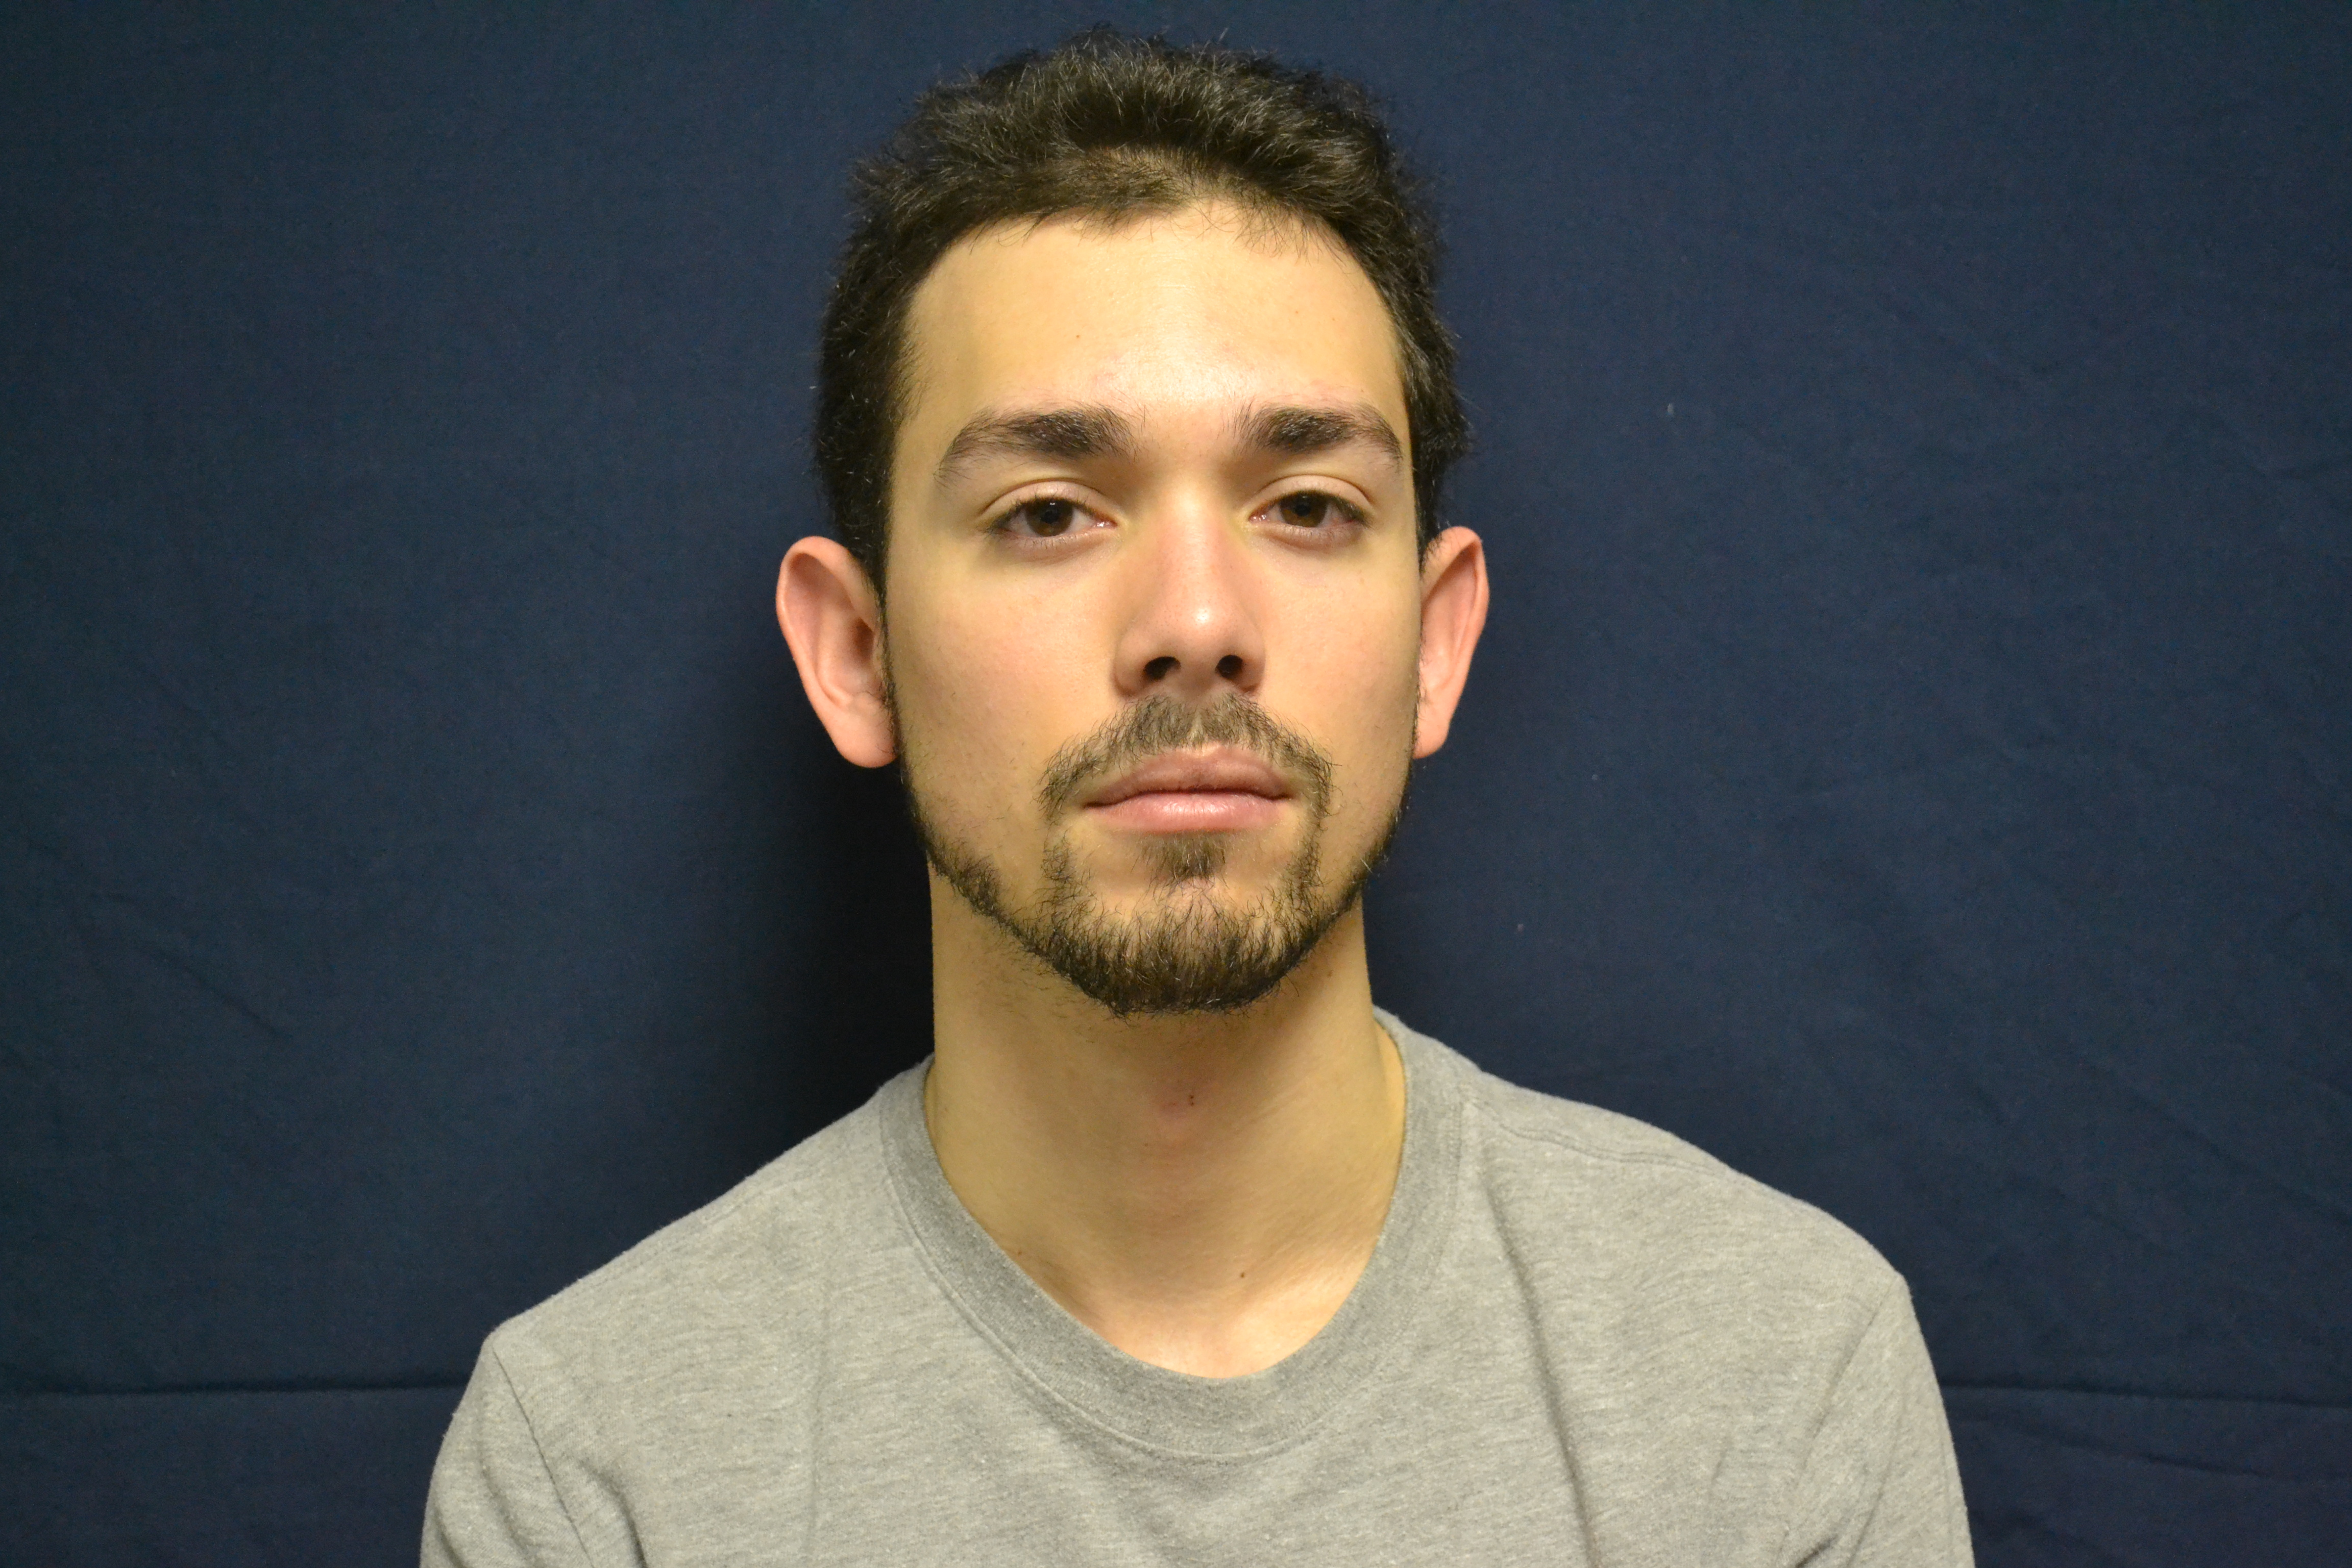
\includegraphics[width=4.1cm]{figures/0.jpg} }}
%     \qquad
%     \subfloat[\centering]{{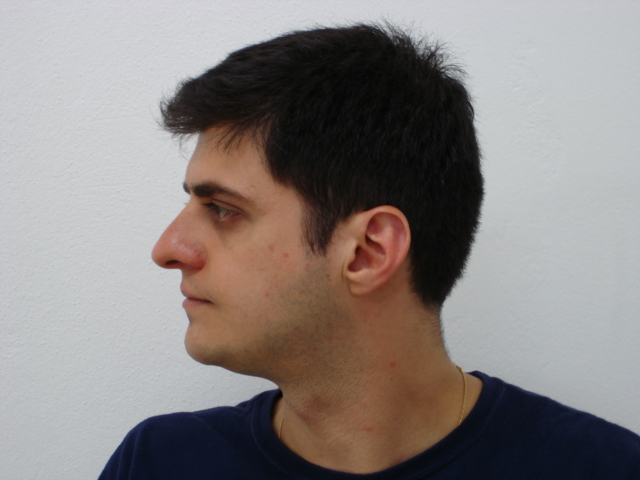
\includegraphics[width=3.65cm]{figures/50.jpg} }}
%     \caption{Facial images from Combined passport alike.}
%     \label{fig:combined_passport_alike}
% \end{figure}
%
\begin{figure}[h]
\centering
    \subfloat
        {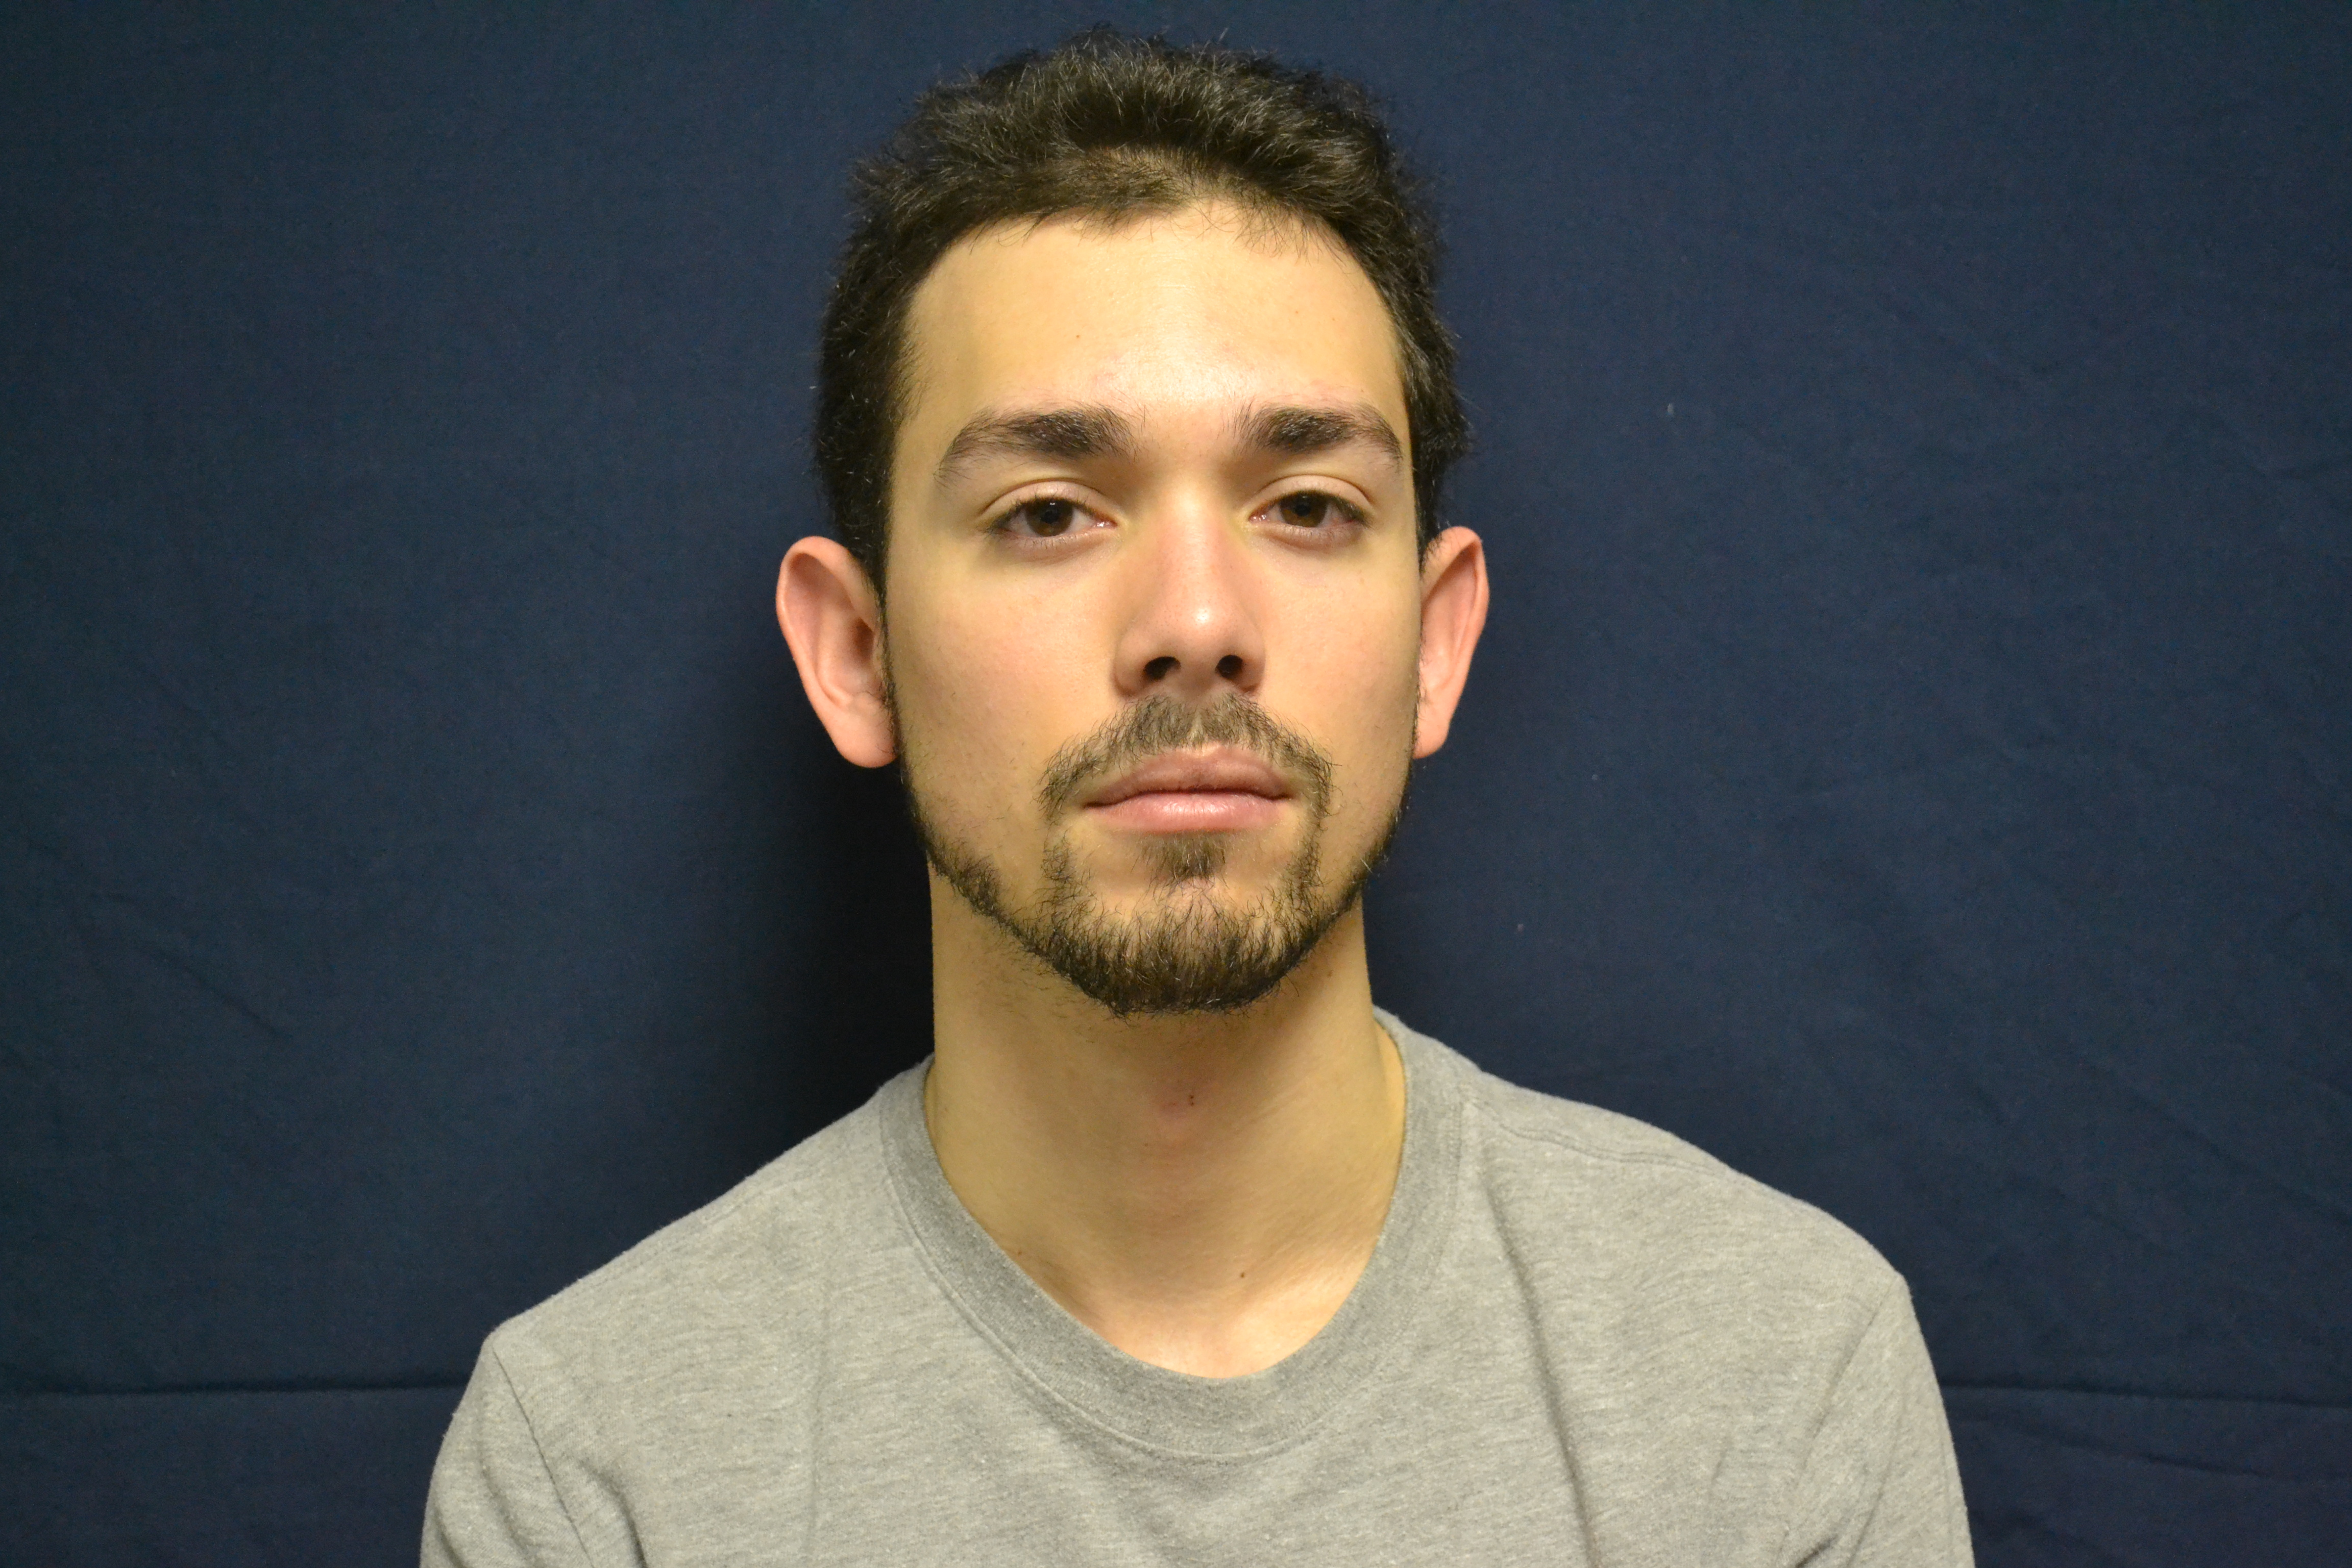
\includegraphics[scale = 0.12]{figures/0.jpg}\hspace{0.42cm}}
    \subfloat
        {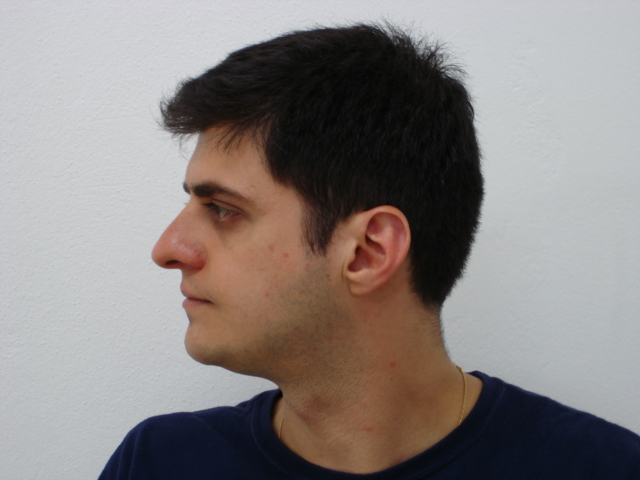
\includegraphics[scale = 0.185]{figures/50.jpg}\hspace{0.42cm}}
    \caption{Facial images from Combined passport alike.}
    \label{fig:combined_passport_alike}
\end{figure}
%
Capture from photo was created by several employees at NTNU and combined with images from the CASIA Face Antispoofing Database \cite{CASIA-FAD}. All 70 images were selfies, taken with different phone cameras. Like Combined passport alike, the people had different poses and facial expression. However, in this dataset, the images by the NTNU employees were photographed in multiple locations on campus, which made the background and lightning vary considerably. The CASIA images were captured from computer screens that would possibly affect the FIQM's evaluation scores. Due to GDPR issues, only images from CASIA are included in Figure \ref{fig:capture_from_photo}.
%
% \begin{figure}[h]
%     \centering
%     \subfloat[\centering]{{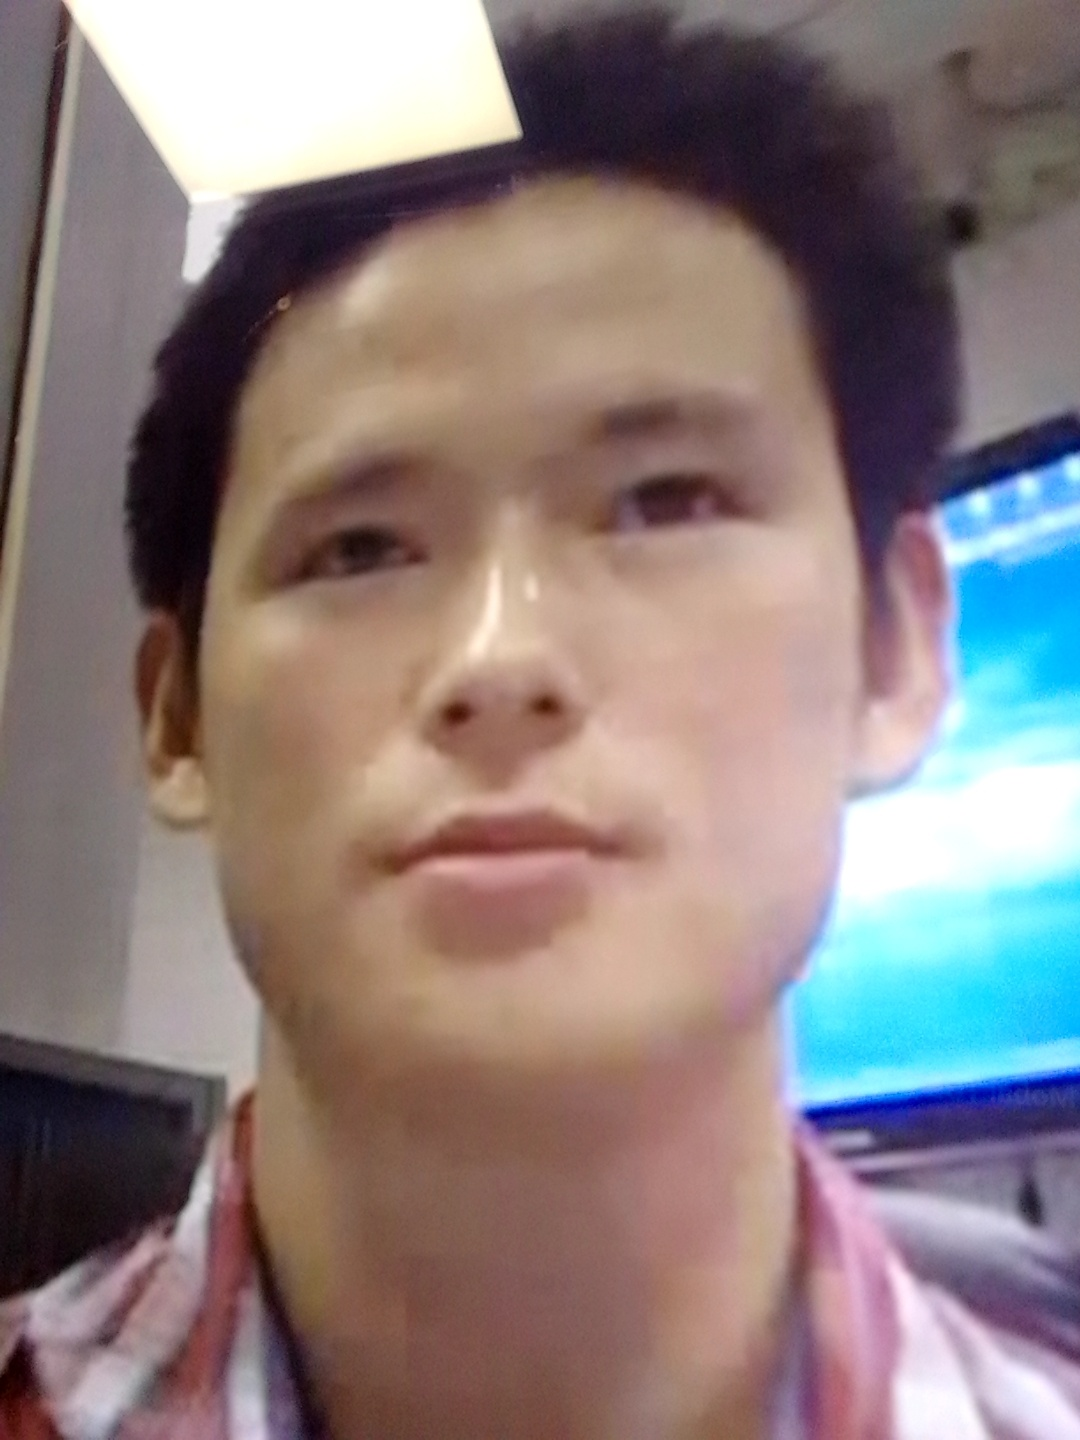
\includegraphics[width=3cm]{figures/1_0.89185.jpg} }}
%     \qquad
%     \subfloat[\centering]{{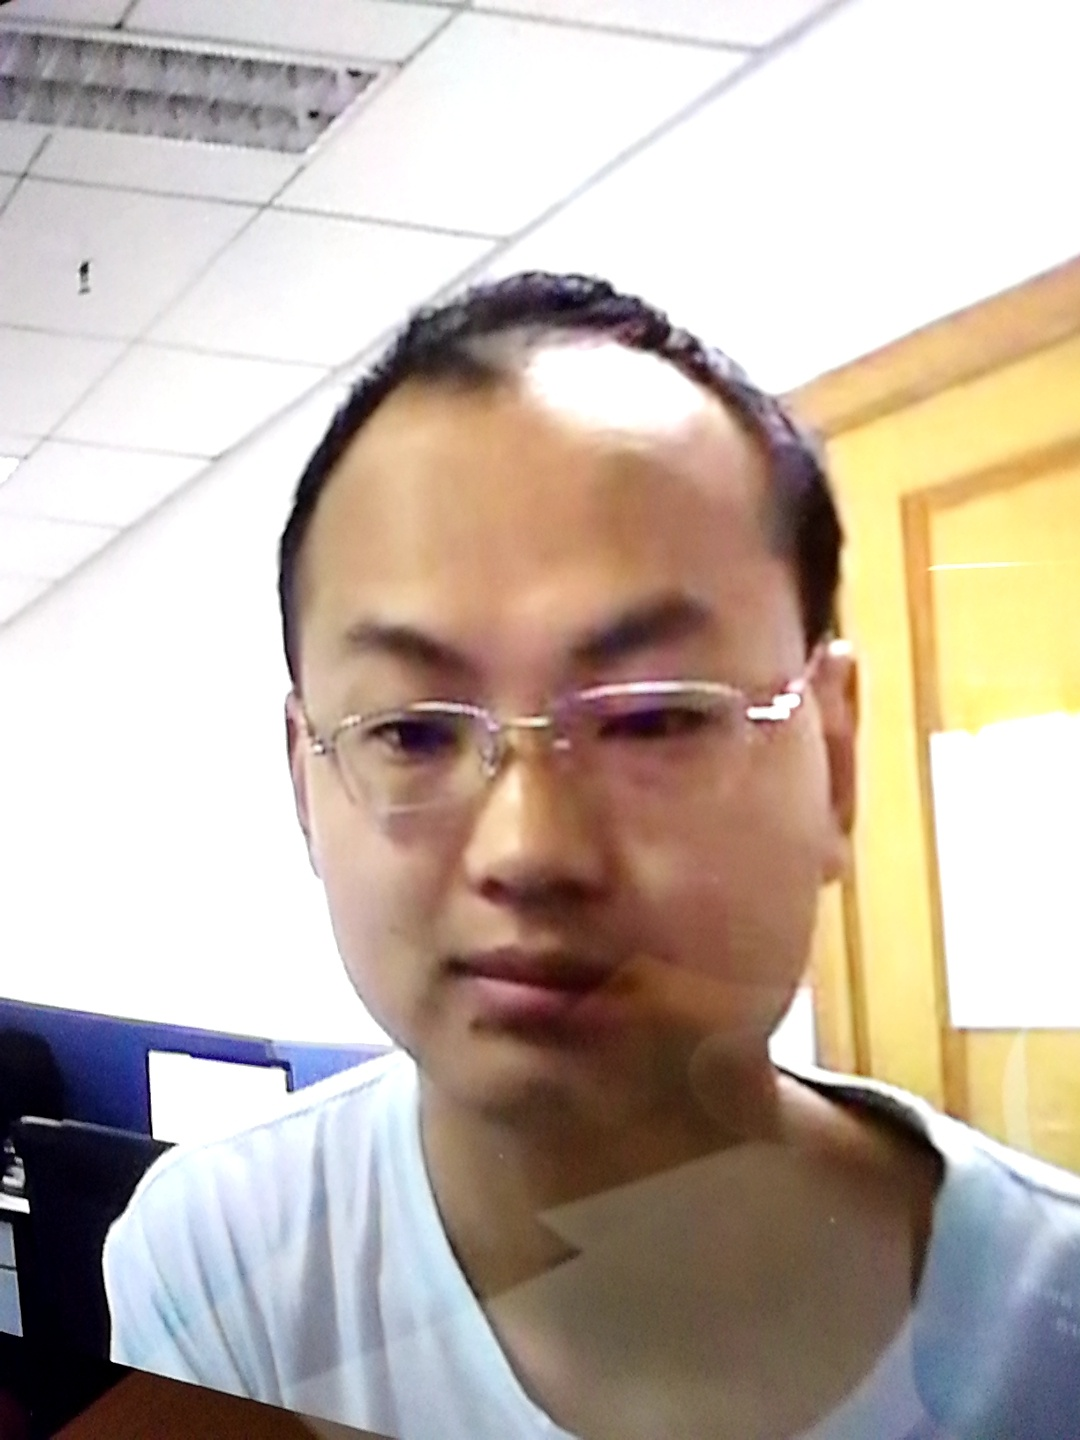
\includegraphics[width=3cm]{figures/5_0.97369.jpg} }}
%     \caption{Facial images from Capture from photo.}
%     \label{fig:capture_from_photo}
% \end{figure}

\begin{figure}[h]
\centering
    \subfloat
        {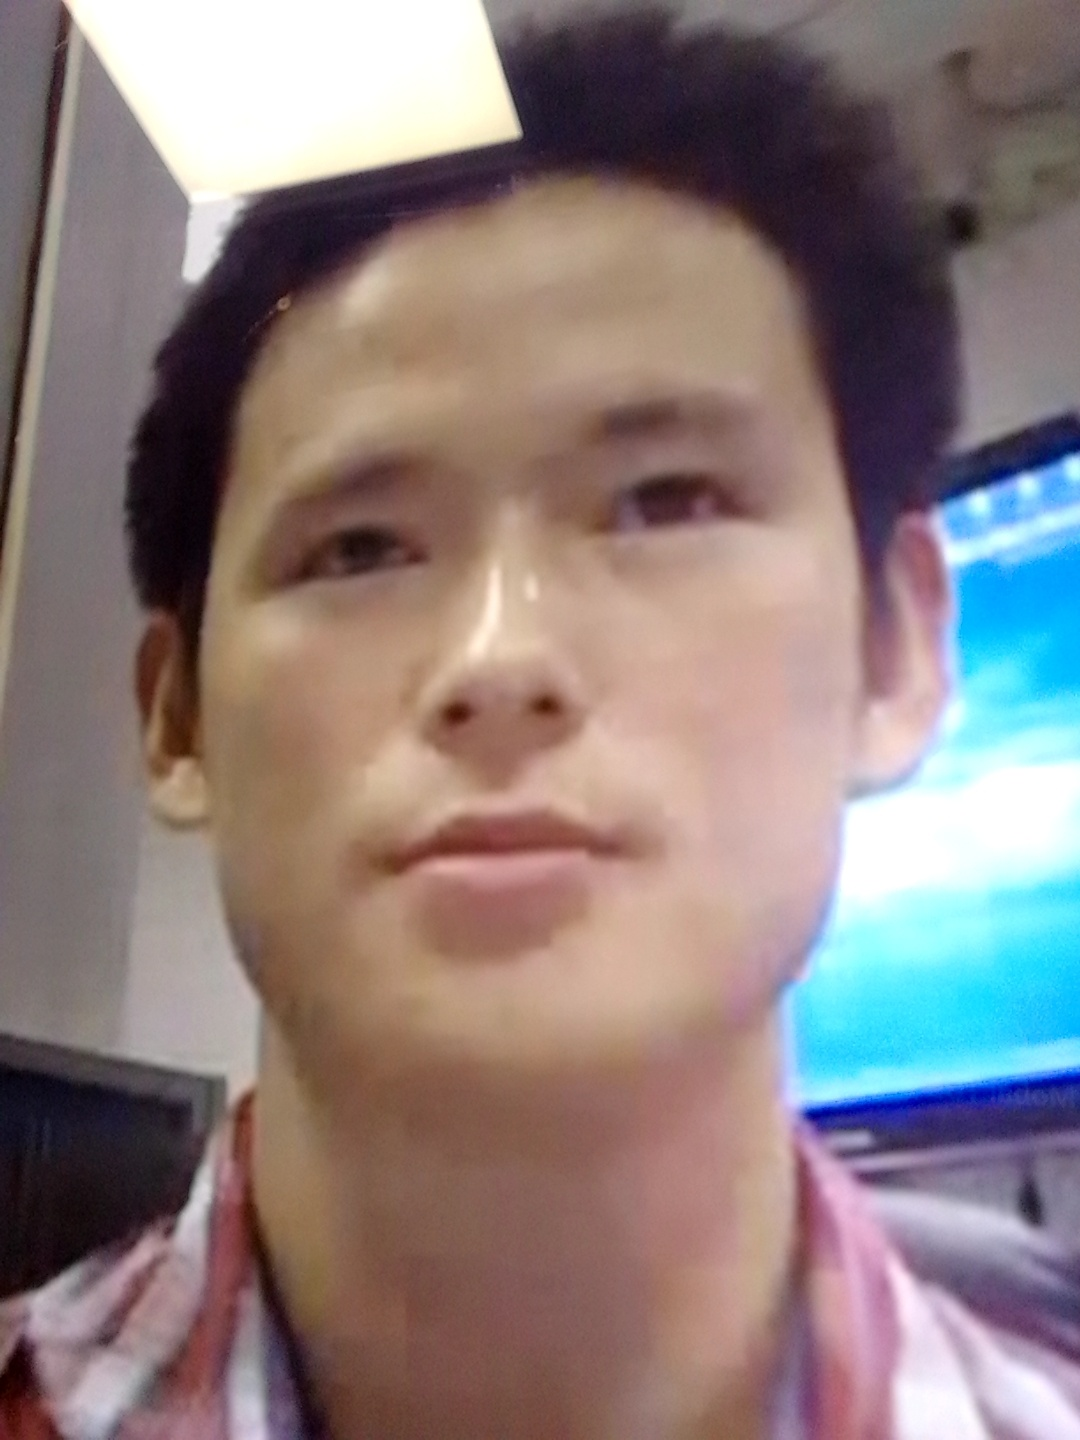
\includegraphics[scale = 0.09]{figures/1_0.89185.jpg}\hspace{0.42cm}}
    \subfloat
        {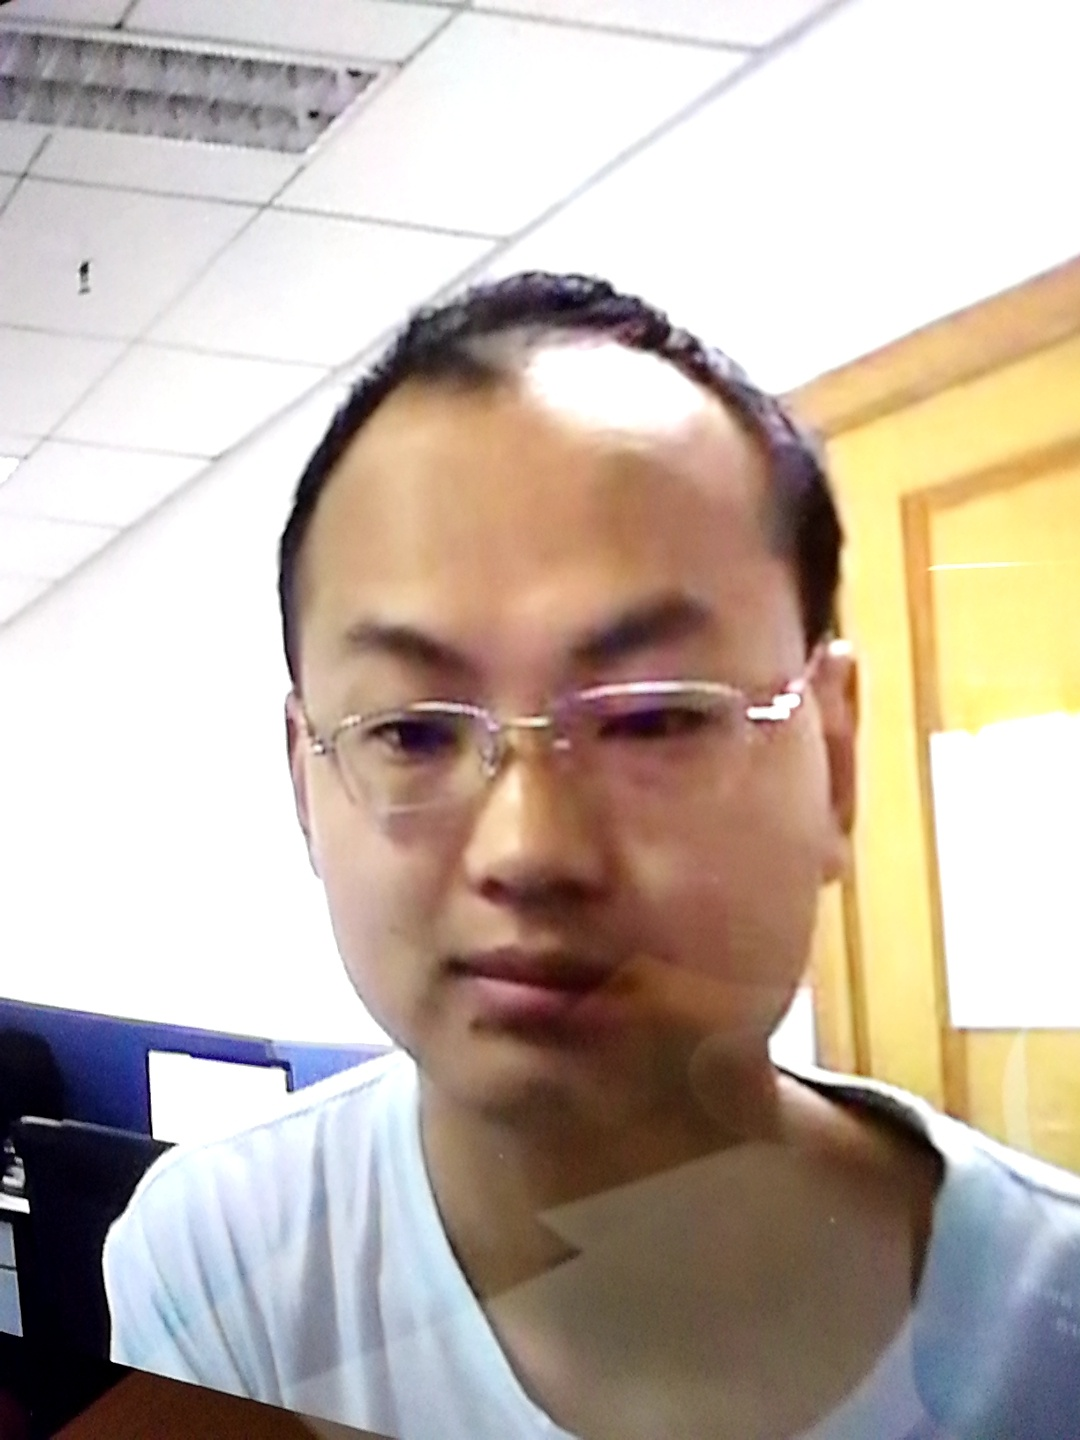
\includegraphics[scale = 0.09]{figures/5_0.97369.jpg}\hspace{0.42cm}}
    \caption{Facial images from Capture from photo.}
    \label{fig:capture_from_photo}
\end{figure}
%
The Selfie dataset was a set of 126 images accessible on the web \cite{selfie-dataset}. The images were selfies of different people at numerous locations: both indoors and outdoors. Given the selfies, the photos were taken with phone cameras and the camera to subject distance was short. A sample from the dataset is shown in Figure \ref{fig:selfie_dataset}. 
%
% \begin{figure}[h]
%     \centering
%     \subfloat[\centering]{{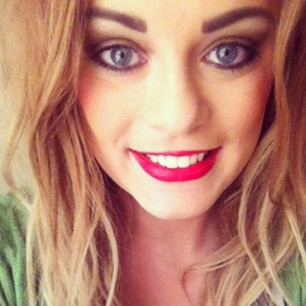
\includegraphics[width=3cm]{figures/10249165_693227110715964_1497214365_a.jpg} }}
%     \qquad
%     \subfloat[\centering]{{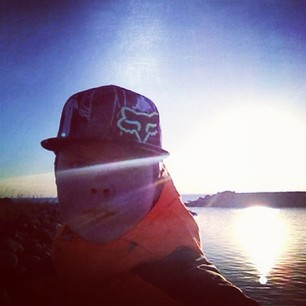
\includegraphics[width=3cm]{figures/10251439_436588196485138_396348425_a.jpg} }}
%     \caption{Facial images from Selfie dataset.}
%     \label{fig:selfie_dataset}
% \end{figure}
\begin{figure}[h]
\centering
    \subfloat
        {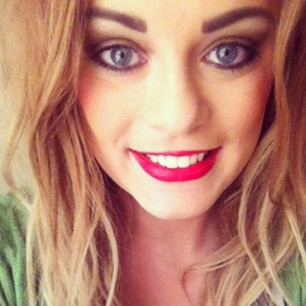
\includegraphics[scale = 0.3]{figures/10249165_693227110715964_1497214365_a.jpg}\hspace{0.42cm}}
    \subfloat
        {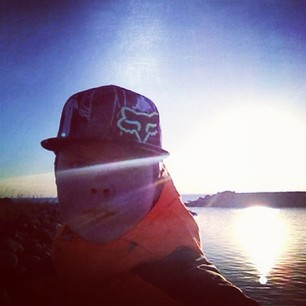
\includegraphics[scale = 0.3]{figures/10251439_436588196485138_396348425_a.jpg}\hspace{0.42cm}}
    \caption{Facial images from Selfie dataset.}
    \label{fig:selfie_dataset}
\end{figure}

%\newpage

\begin{table}[h]
\caption{Information about all datasets used in the project.}
\resizebox{\textwidth}{!}{%
\begin{tabular}{|p{4cm}|p{4cm}|p{4cm}|p{4cm}|} 
\hline
\textbf{Dataset name} & \textbf{Number of images} & \textbf{Captured with} & \textbf{Distortions}  \\ \hline
Combined passport alike & 98 & Nikon D3100 & Exposure \\ \hline
Captured from photo & 70 & Mobile phone & N/A \\ \hline
Selfie dataset & 126 & Mobile phone & N/A \\ \hline
Norwegian Facial Collection & 450 & Apple Iphone 8 \newline Apple Iphone 11 \newline Motorola Moto G5S Plus & Compression \newline Blur  \newline Noise \newline Face mask coverings \newline Oblique angles \\ \hline
\end{tabular}%
}
\label{table:DatasetInformation}
\end{table}

\section{Our Subjective Experiment}
\label{sec:OurSubjectiveExperiment}
In our subjective experiment, observers were asked to grade facial images according to the criteria described in Section \ref{sec:intromanual}, and assigning these images in five categories: poor, bad, fair, good and excellent. We did not chose the rank order system, because comparing multiple images would be challenging and time consuming for the observers. The experiment was separated into three sessions with a five-minute time break between each session. The duration of the subjective experiment was estimated to take approximately 45 minutes. Each session included images from the three datasets which were equally distributed among the sessions. For us, it was important to randomize the facial images to prevent observers getting biased towards one face. The subjective scores were collected from 15 observers - both experts and non-experts. Due to the GDPR, we only asked the observers' gender and if they were experts or not in this field. Out of the 15, 13 were men and two were women. Seven observers were experts, and eight were non-experts. Six experts were men, and one woman. Seven non-experts were men, and one non-expert was a woman. 
%
\subsection{Instruction Manual}
\label{sec:intromanual}
When conducting the subjective experiment and collecting the ground truth data, we first needed to provide a detailed instruction to the observers. This was especially important in the case of non-experts who were not familiar with the task. Such an instruction manual will also allow us to provide a uniform understanding for the observers on how they should perform the subjective experiment. Thus, an experiment instruction manual was made. The instruction manual is included in Appendix \ref{app:survey-instructions} 

The first clarification we had to convey to the participants, was the meaning of face image quality. Both experts and non-experts would have different perceptions in terms of face image quality and we had to clarify all factors affecting face image quality. The most clear and effective way to train the observers was to visualize examples of rated images like they would do in the subjective experiment. We created five example lineups with selfies of ourselves. Those facial images included most issues affecting the quality of an image. 

\begin{figure}[h]
\centering
    \subfloat[Poor]
        {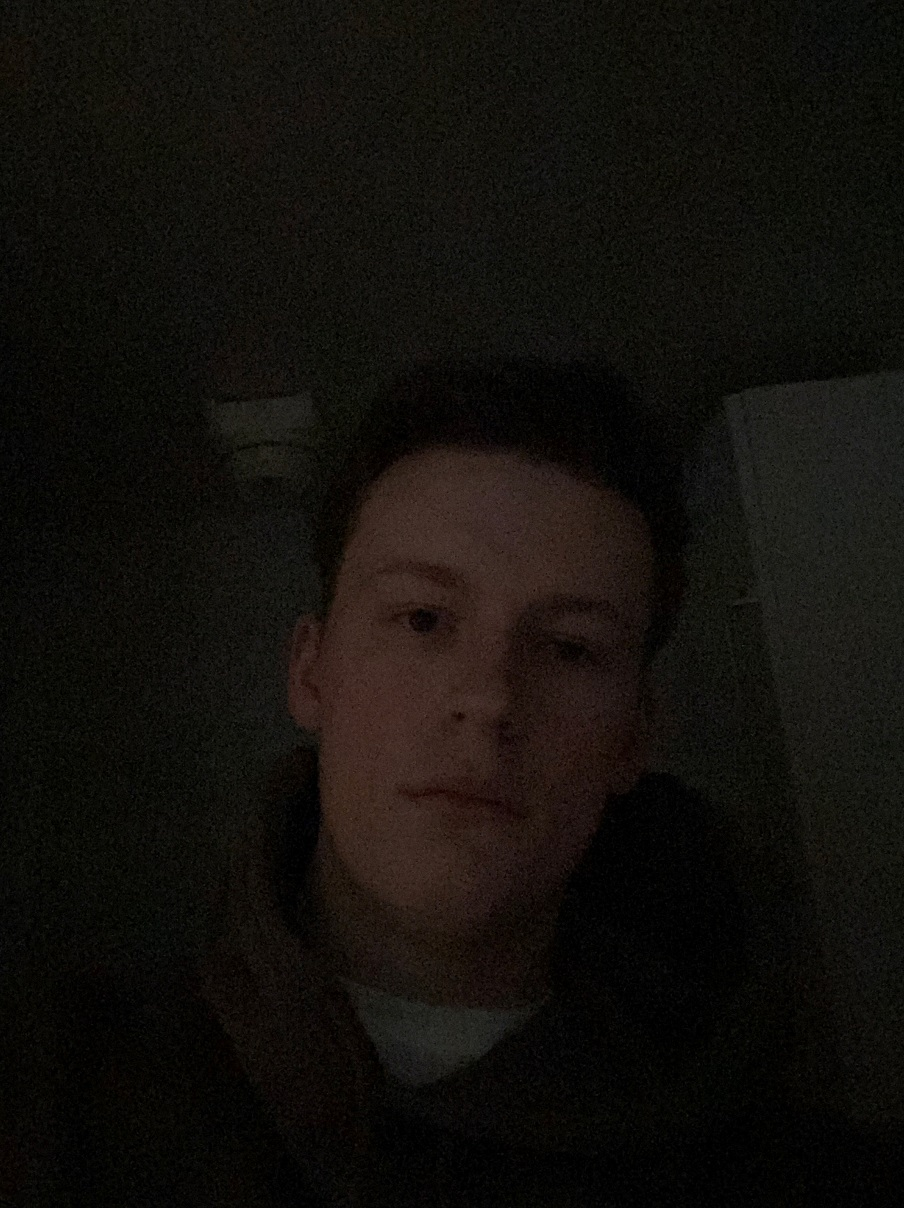
\includegraphics[scale = 0.0825]{figures/lineup1.png}}
    \subfloat[Bad]
        {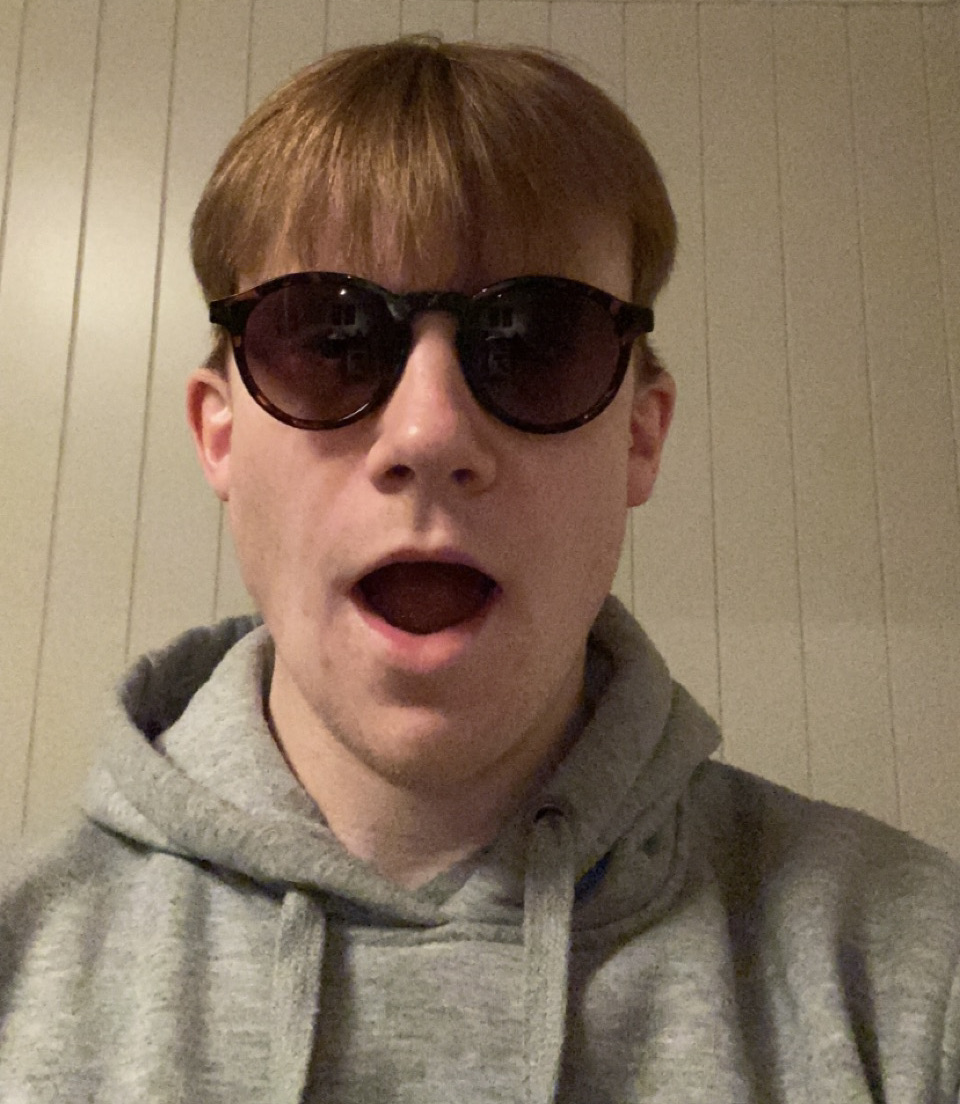
\includegraphics[scale = 0.0901]{figures/lineup2.png}}
    \subfloat[Fair]
        {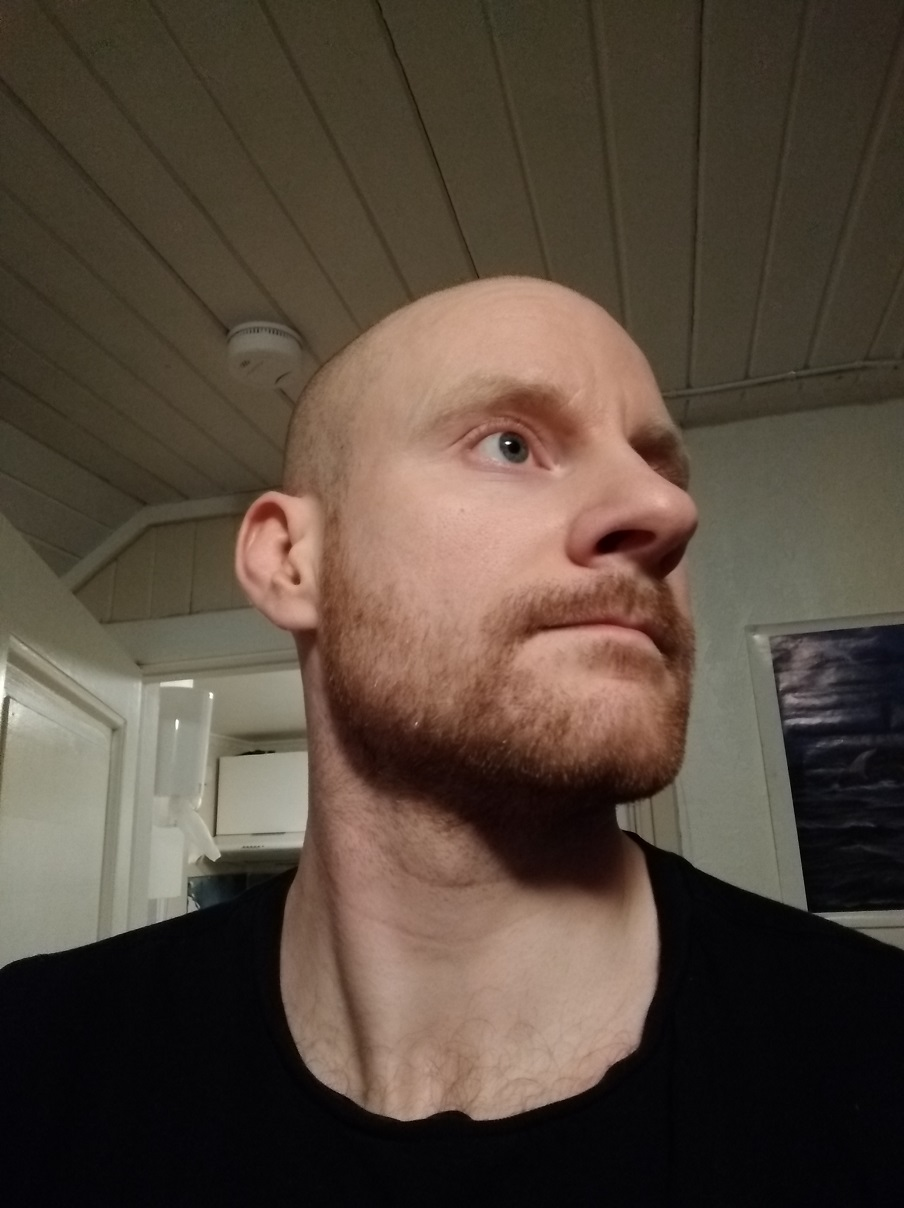
\includegraphics[scale = 0.0825]{figures/lineup3.png}}
    \subfloat[Good]
        {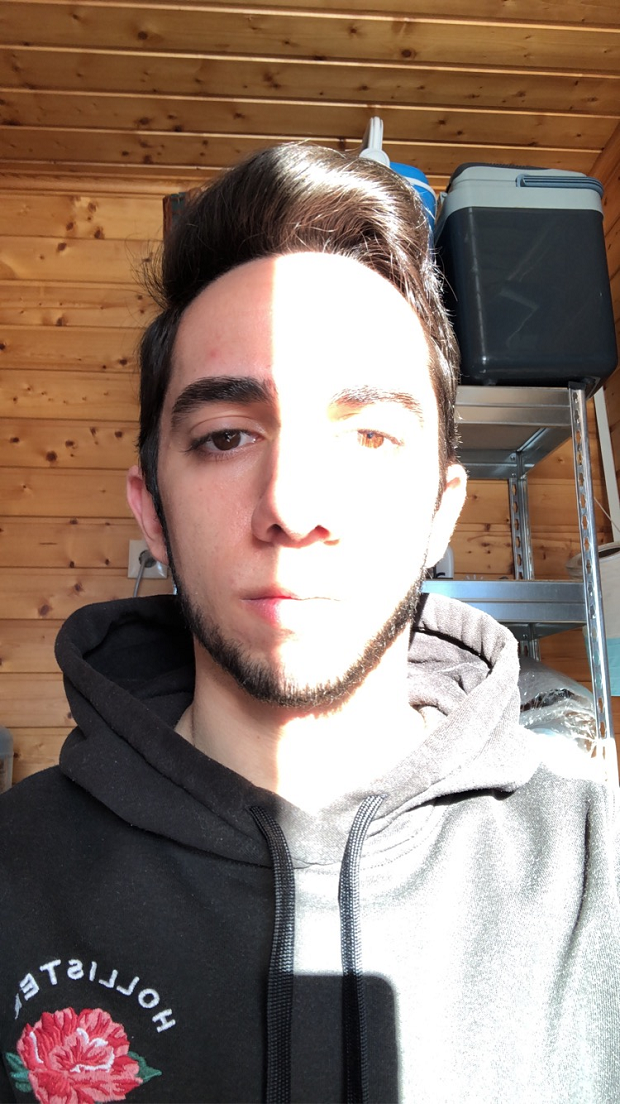
\includegraphics[scale = 0.09]{figures/lineup4 - Copy.png}}
    \subfloat[Excellent]
        {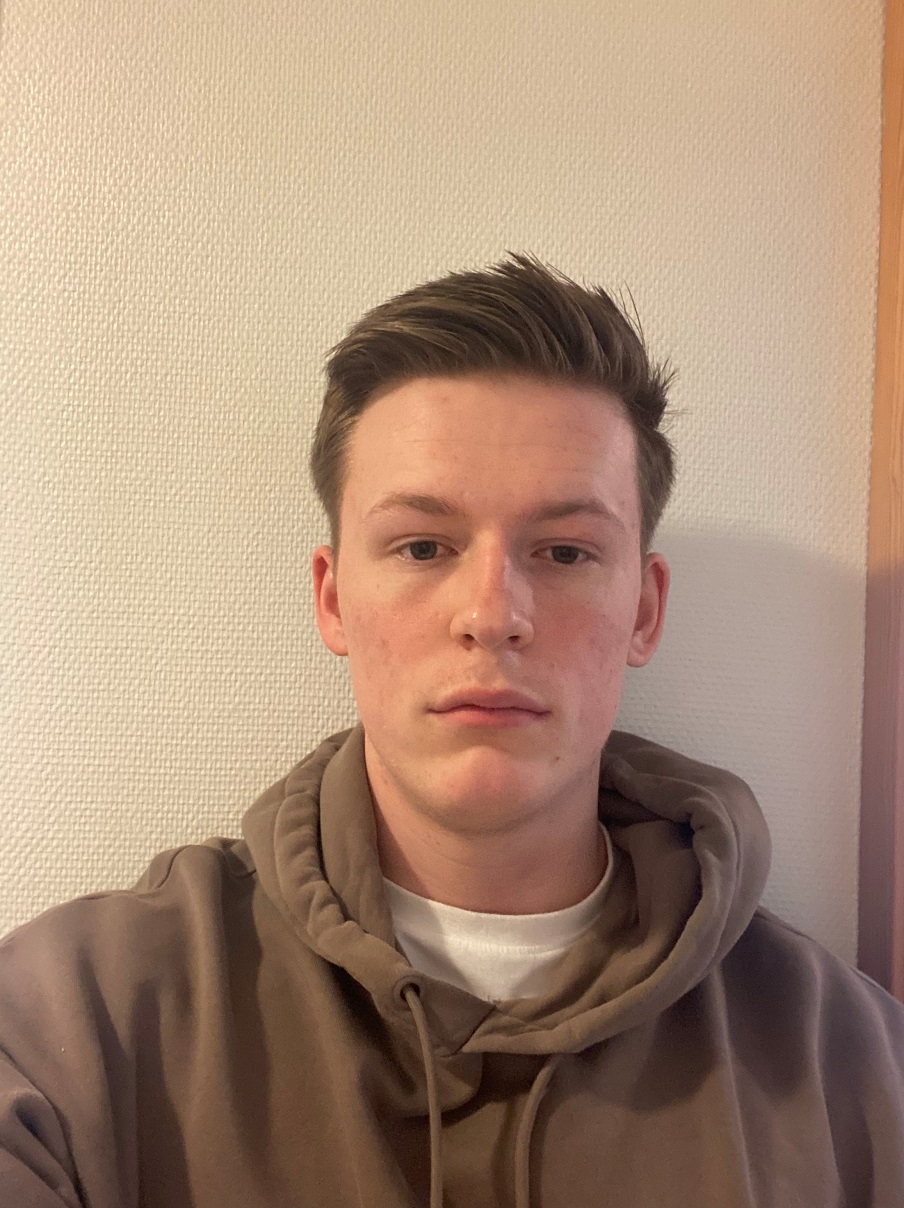
\includegraphics[scale = 0.0825]{figures/lineup5.png}}
    \caption{A lineup from the experiment instruction manual and their quality ratings.}
    \label{fig:example-manual}
\end{figure}

The lineup images in Figure \ref{fig:example-manual} is a sample lineup provided to the observers to guide them on how to rate the images. In the experiment however, some participants found it harder to rate the experiment images, because they included several image properties to take into account.

\subsection{Choice of Subjective Experiment Platform}
\label{subsection:choicesoftware}
A decision we thought would be easy, but ended up being challenging and time consuming was selecting the platform in which we would run our subjective experiment. There were a number of possible platforms for conducting the subjective experiment. However, we had to bare in mind the factors described in Section \ref{sec:SubjectiveAspects} in our selection. One experiment platform we found interesting was Survey Monkey. The main reason we abstained from Survey Monkey was their demand of creating a yearly subscription to use functions such as displaying questions in random order. We even asked for a four month subscription without luck. Another platform we found appropriate was Survey Legend, a subjective experiment platform perfectly suitable for images. It included many functions we needed, except enabling questions to be ordered randomly for each observer. Therefore, we unfortunately had to abort Survey Legend as well. 

After consulting with our supervisor, we ended up arranging the subjective experiment in QuickEval \cite{QuickEval} - a experiment platform developed by NTNU. The platform provided every functionality we needed such as category judgment and random order of questions. Each image was positioned in the center of the screen on a neutral background, we also too care every image in the datasets were similar in size. Our psychometric experiment was available for everyone to participate, but specific employers at Mobai and NTNU were specially invited. This was so we can collect answers from experts in the field. QuickEval displayed statistics in the application gradually as people responded to the experiment. The statistics data was also downloadable as a CSV, HTML or Excel file. 
Using QuickEval as a experiment platform ended up being a good choice because it was created by NTNU and we had a close relationship with the developers. When an issue occurred, we submitted that issue and communicated directly with a developer resulting in the issue to be fixed quickly. 

\section{COVID-19 Pandemic Implications}
Due to the ongoing \acrshort{covid19} pandemic, limitations with the subjective experiment occurred. For example, we did not have the opportunity to create a controlled environment and invite the participants to complete the subjective experiment there. Ideally, such a controlled environment would be a well-lit room with good air quality, timed breaks between the sessions and a computer with specific screen settings for all participants to complete the experiment on. The Norwegian Colour and Visual Computing Laboratory in NTNU Gjøvik would be a perfect environment that could be standardized according to \acrfull{cie} publications, but unfortunately this was not achievable given the COVID-19 restrictions. For that reason, all the participants completed the subjective experiments in an uncontrolled environment using their own computers with their custom screen resolution and lighting conditions. While factors such as the monitor brightness and color temperature and even the participants distance from the monitor as well as the illuminance of the room, plays an important role. We believe that due to the nature of our experiment (collecting ground truth data) the results collected in our work would be reliable and scientifically accurate. We should point out that while when it comes to evaluating the general quality of the image parameters such as the viewing condition and/or emotions of the observers play an important role this is normally not the case in the type of subjective data we were collecting. 

\raggedbottom %Fikser problemer med white space

\section{What Went Wrong?}
Despite conducting the subjective experiment in uncontrolled environments, the accomplishment of the experiment was successful. Due to the targeted invitation we sent to observers, a reasonable number of participant provided us with their subjective evaluation in a short time which resulted in us having more time analyzing the data. Since it was our first time creating this kind of experiment, some experiment aspects were left out of the consideration that could be important. The main flaw with this experiment, was the lack of information about observes' characteristics, especially color blindness. Research show that \acrfull{cvd} affects eight percent of men and 0.5 percent of women in the world \cite{colorblindness}. Given that 87 percent of the observers participating in our experiment were men, there was a possibility that color blindness existed among the observers. People with a type of color blindness have the ability to discern colors to a lesser degree than people with normal color vision. Therefore, this will affect the way they assess the facial images which is the reason why they are not contemplated as optimal observers \cite{Xphdthesis}. A good solution would be to test all participants with standardized color vision tests like an Ishihara test \cite{Ishihara} or a Cambridge color test \cite{CambridgeColorTest}.   

Another experimental aspect we systematically excluded was to provide the observers with a question during the experiment. We had initially planned for the experiment to consist of a precise question to minimize any doubt the observers could have. A criteria we had in mind was: ``How well is the face recognizable?''. We felt this question could confuse the observers given that the word recognize often refers to knowing a person in advance. Since most participant would not know any of the subjects in the datasets in advance, we dropped that question. However, since we created an instruction manual with aspects that affected the face quality, we figured the observers would have a clear understanding of what was to be rated. But looking back, a question like: ``How visible is the face according to the criteria described in the instruction manual?'', could have been beneficial to clear up any misunderstandings.   

\section{Creating Our Own Dataset}
\label{sec:ownData}
When working with machine learning and AI in the context of face recognition, the probability of using one of the famous pre-curated Labeled Faces in the Wild (LFW) datasets are highly likely. Conditions such as poor lightning, extreme poses and face coverings are somewhat lacking in LFW and these are all important aspects for Mobai´s face recognition system. This provided us with the opportunity to collect a specialized dataset designed to fit Mobai´s needs which led to the proposal of a new dataset. This initiative was positively received by Mobai.

The idea to collect a new dataset came about when the team was discussing flaws with the Selfie dataset. Mobai´s definition of face quality is, as mentioned in Section \ref{sec:setup}, originally based on ISO 29794-5 and ICAO Doc 9303 Part 3. Based on those definitions, one could argue that the images in the Selfie dataset did not fulfill the criteria. A significant part of the images in the Selfie dataset are of faces that either are way off-centered, too zoomed in or a combination of both. We figured it could be valuable for Mobai to have a new dataset aligned with certain criteria they valued. 

\subsection*{Creation Process}
We had initially taken a few images of ourselves which were used for the instruction manual, illustrated in Figure \ref{fig:example-manual}, to the subjective experiment. These were included when we started collecting images for the dataset. We came to the conclusion that each day, starting 1. March and ending 15. April, we would capture at least five selfies of ourselves every day. This would result in a total of 250 images of each member. We ended up capturing 1172 images. With this amount of images, there were a lot of repetitive facial images. Therefore, we selected 250 images from the collection. In addition, we selected 50 of these images and added different distortions (described in detail in Section \ref{sec:secondse}) on them. The whole dataset consisted of 450 images. Our dataset is relatively large in size in comparison to the combined dataset used in our experiment. Some of the images are similar to the Combined passport alike dataset in regards to pose, but our dataset includes several varieties and specialized conditions which will be presented below. We chose to name our data set Norwegian Facial Collection (NFC).

All the images were captured using both the front and back camera of our mobile phones. This lead to our dataset containing images of varying resolution, given that our phones were not of the same type. The phones used for the dataset collection were:
\begin{itemize}
    \item Apple iPhone 8 
    \item Apple iPhone 11 (2 units)
    \item Motorola Moto G5S Plus 
\end{itemize}
%
These had different camera specifications with the front cameras ranging from seven to 12 megapixels and the back cameras ranging from 12 to 13 megapixels. While the difference in image resolution was very minor making it barely noticeable to the user, it still is able to simulate what FIQMs will need to address in real life applications. 

\subsection{Distortions}
Our dataset was inspired by the three datasets introduced in Section \ref{sec:datasets}, but was unique because elements like camera angles and face masks were represented. During our image collection, we gathered examples of our faces with: 
%
\begin{itemize}
    \item Different lightning conditions.
    \item Different facial expressions and head poses.
    \item Different face and head coverings. 
    \item Different camera angles and camera tilts.
    \item Different backgrounds.
    \item Different distortions such as compression, blur and noise.
\end{itemize}

A crucial consideration was to gather a high number of images that cover a wide range of varying qualities. facial images of bad quality were equally as important as excellent quality facial images, because machine learning algorithms such as FIQMs rely on diversified images to learn.  

\subsubsection*{Face Masks}
One of the two significant aspects of our dataset was the inclusion of face mask images. The usage of face masks has drastically changed people's everyday lives across the globe. This is especially true in western society, since face masks were almost non-existent in public areas before the corona pandemic. Seeing that face masks became a normal part of peoples lives, we figured Mobai´s face recognition system would have limited images with face masks to test their FIQMs. 
To achieve a variety of face mask images, we altered the coverage of the face masks. The common way to wear a face mask is for it to cover your mouth and nose. Some of the images were captured with those aspects taken into consideration, but a significant number were captured with the masks covering less of the face, as shown in Figure \ref{fig:masks}. All those images were expected to receive noteworthy different scores by ISO Metrics and FaceQnet because the visibility of the faces were dissimilar.  
\begin{figure}[h]
\centering
    \subfloat
        {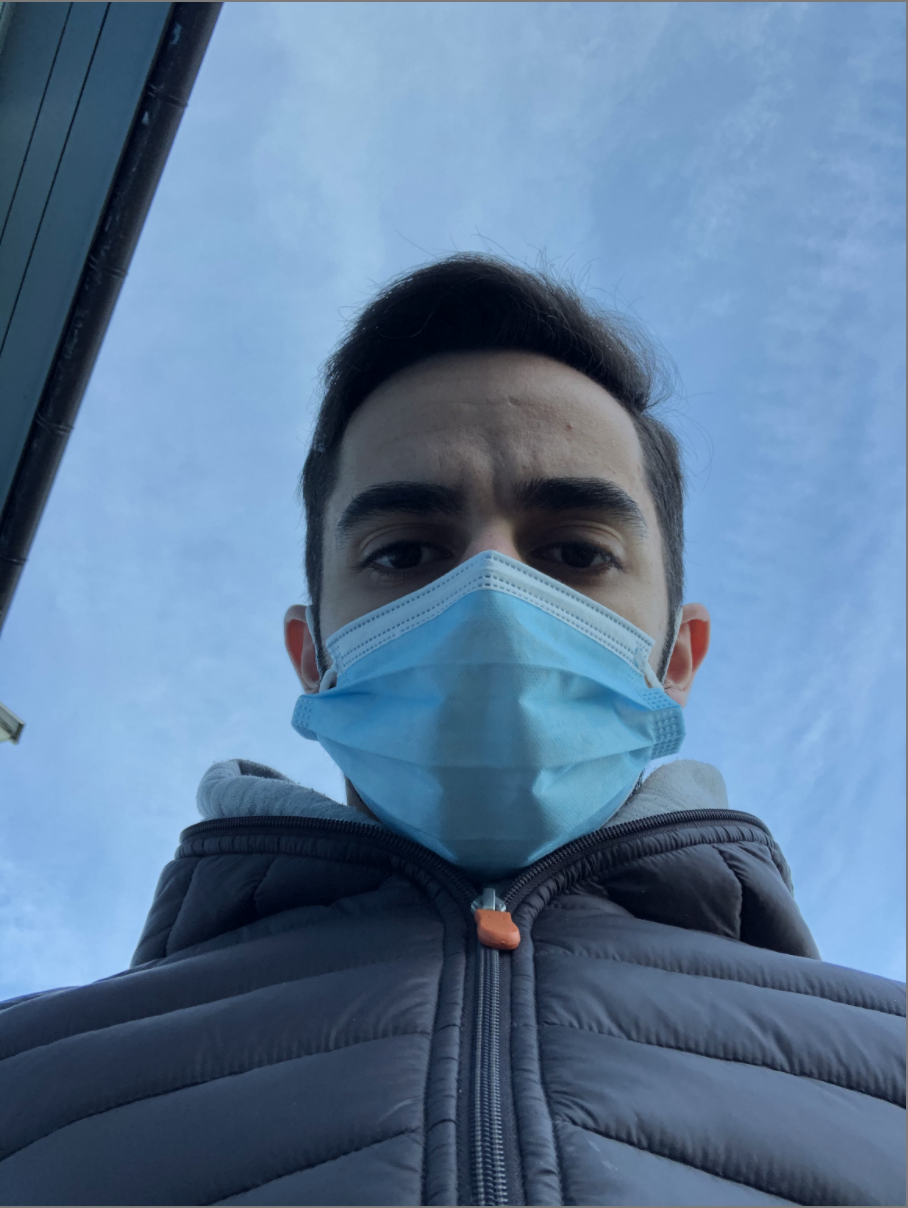
\includegraphics[scale = 0.18]{figures/1133.png}\hspace{0.42cm}}
    \subfloat
        {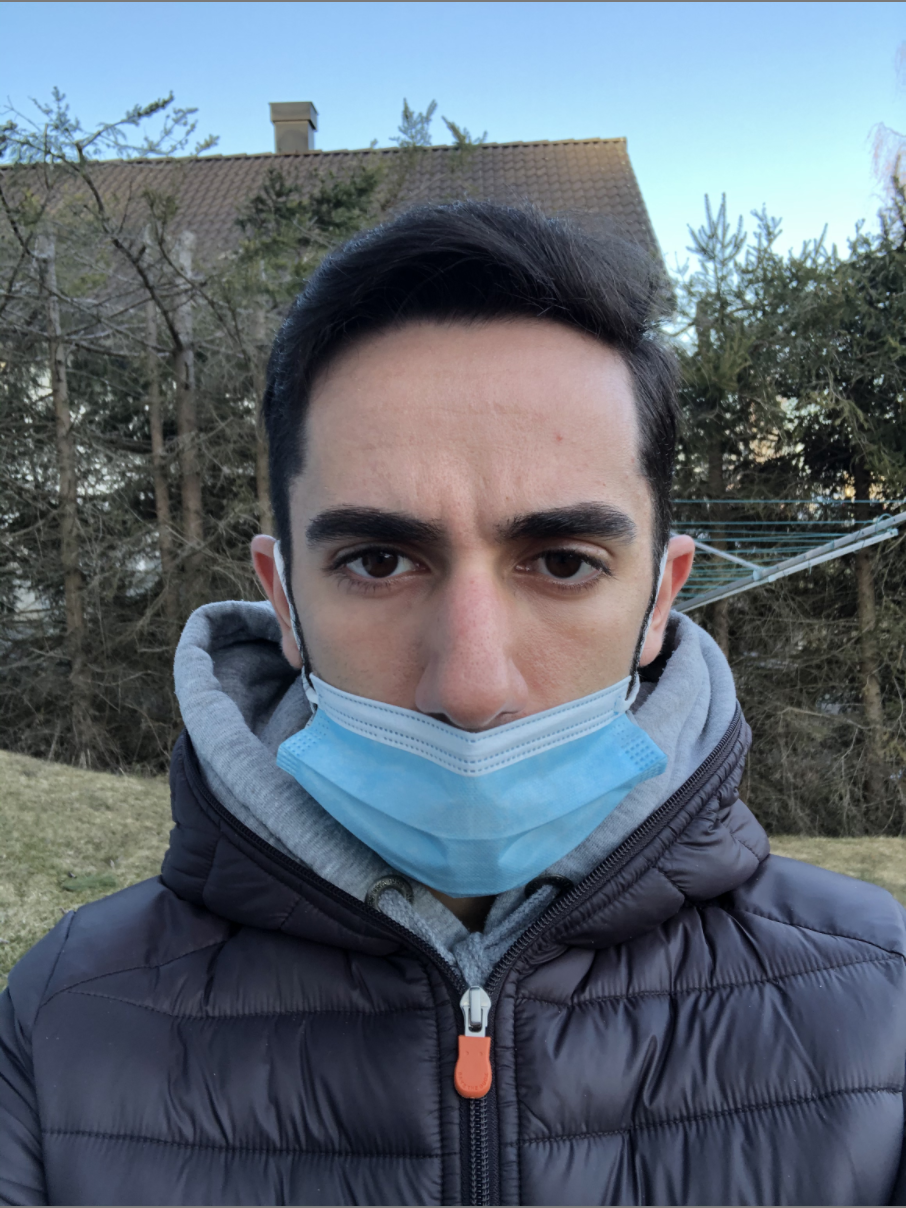
\includegraphics[scale = 0.18]{figures/940.png}\hspace{0.42cm}}
    \subfloat
        {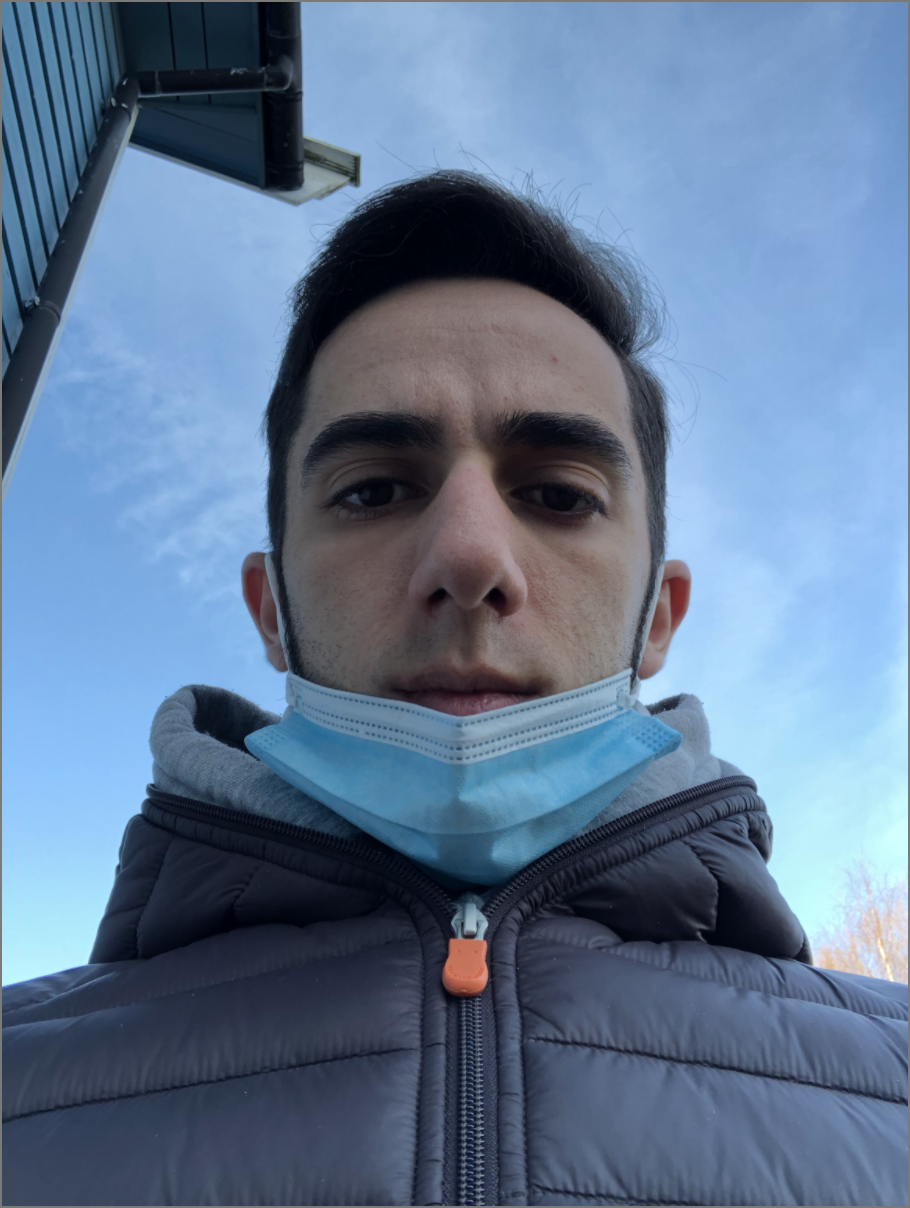
\includegraphics[scale = 0.18]{figures/1110.png}\hspace{0.42cm}}
    \subfloat
        {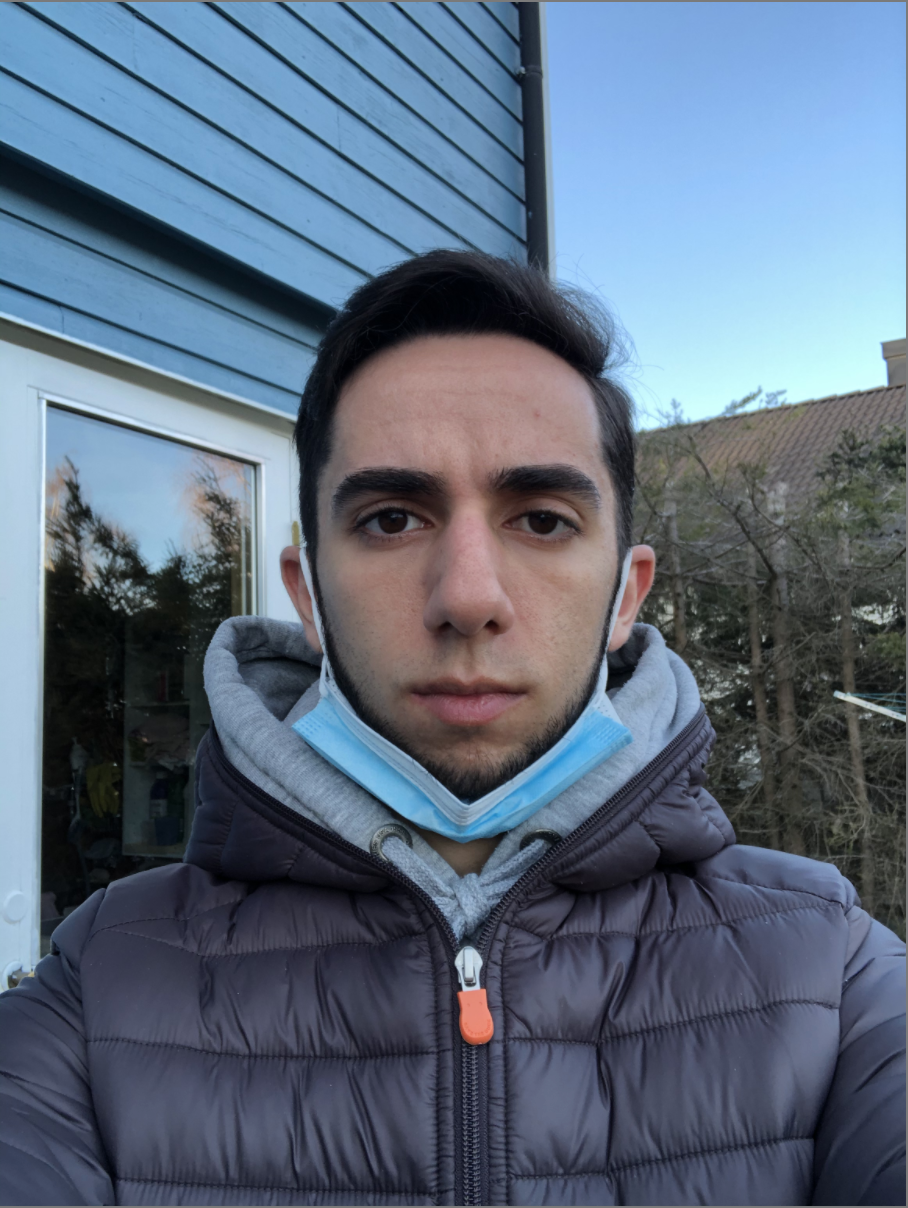
\includegraphics[scale = 0.18]{figures/1152.png}\hspace{0.0cm}}
    \caption{Different face masks usage.}
    \label{fig:masks}
\end{figure}

\subsubsection*{Camera Angles}
The other important contribution to our dataset, was that we experimented with different camera angles, also known as ``oblique angles'' or ``Dutch angle''. These types of images involves angling the camera at an oblique angle on its roll axis, which produces images where the viewpoint is similar to angling one´s head to the side. Images like these create a form of disorientation because the camera has been rotated relative to the horizon of an image. This type of disorientation can be perceived by humans, but whether the FIQMs react differently towards these type of images is yet to be seen. For that reason, we wanted to look into oblique angle facial images and see if the FIQMs produce significantly different scores solely based on the camera angle. 

\begin{figure}[h]
\centering
    \subfloat
        {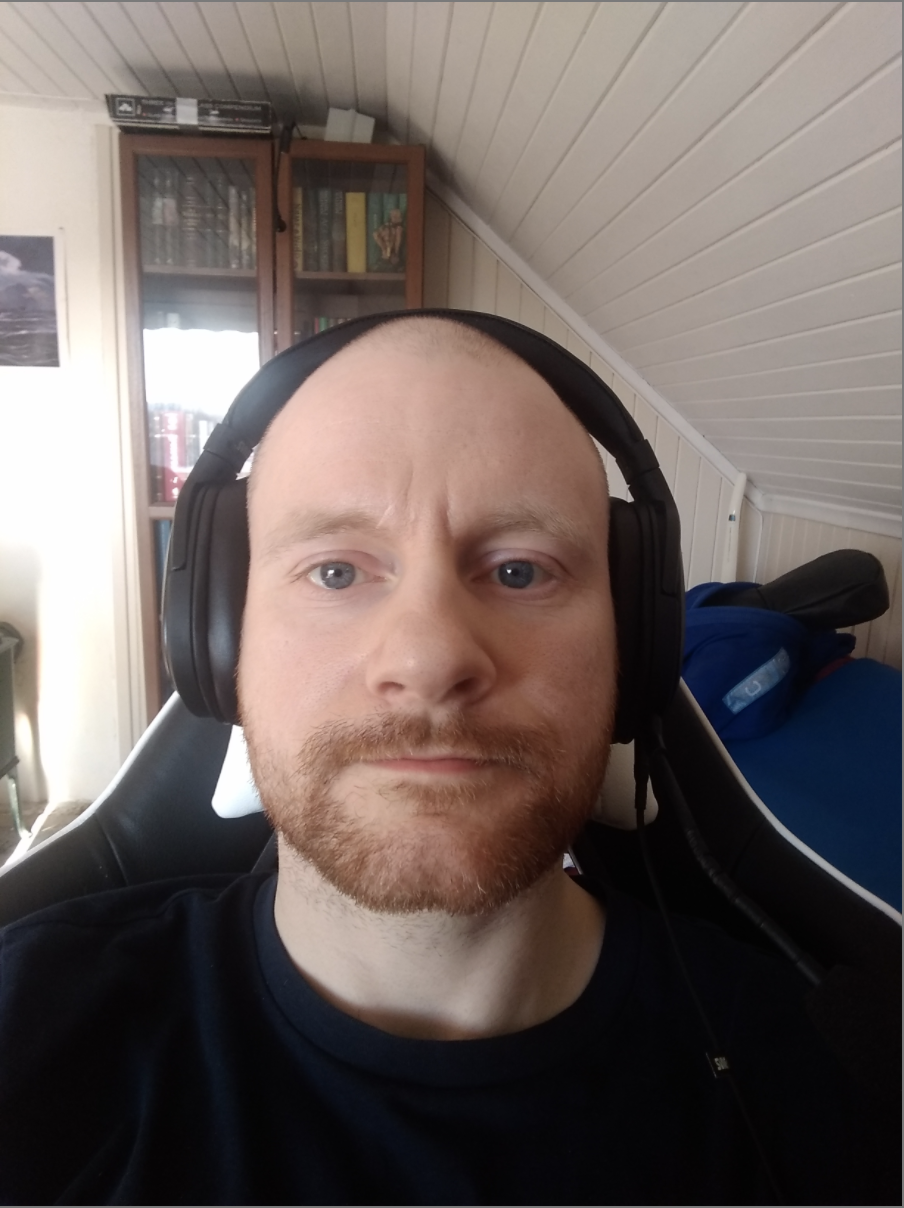
\includegraphics[scale = 0.2]{figures/0368.png}\hspace{0.4cm}}
    \subfloat
        {
\includegraphics[scale = 0.2]{figures/0367.png}\hspace{0.4cm}}
    \subfloat
        {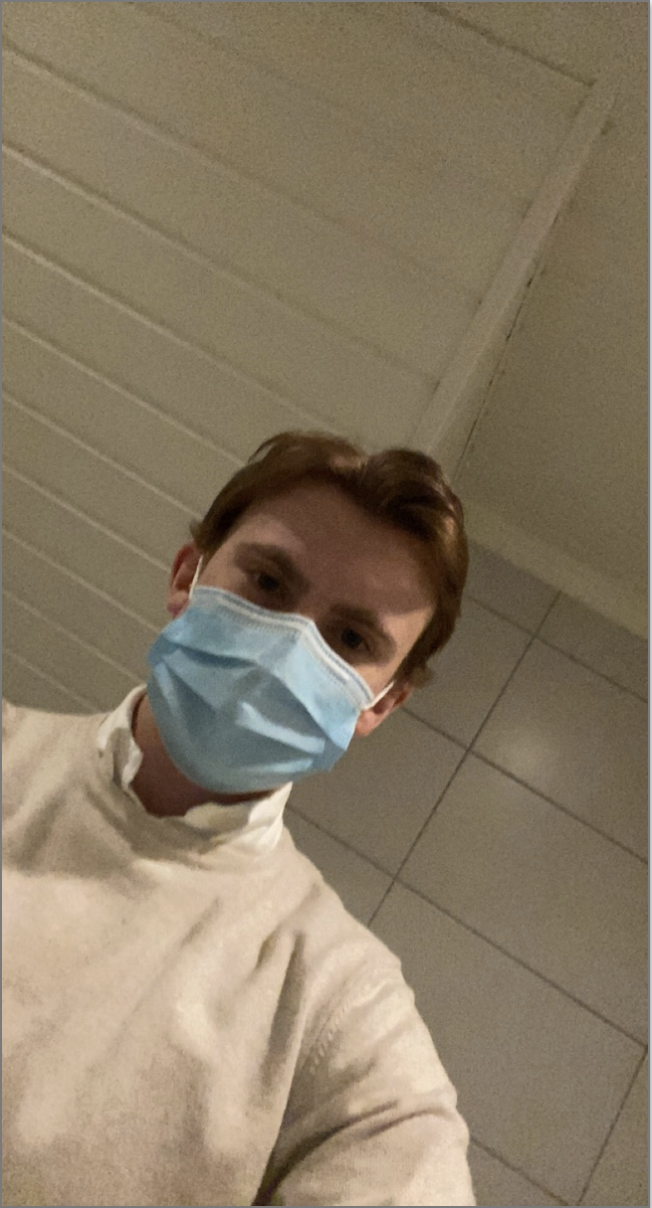
\includegraphics[scale = 0.2]{figures/0129.png}\hspace{0.4cm}}
    \subfloat
        {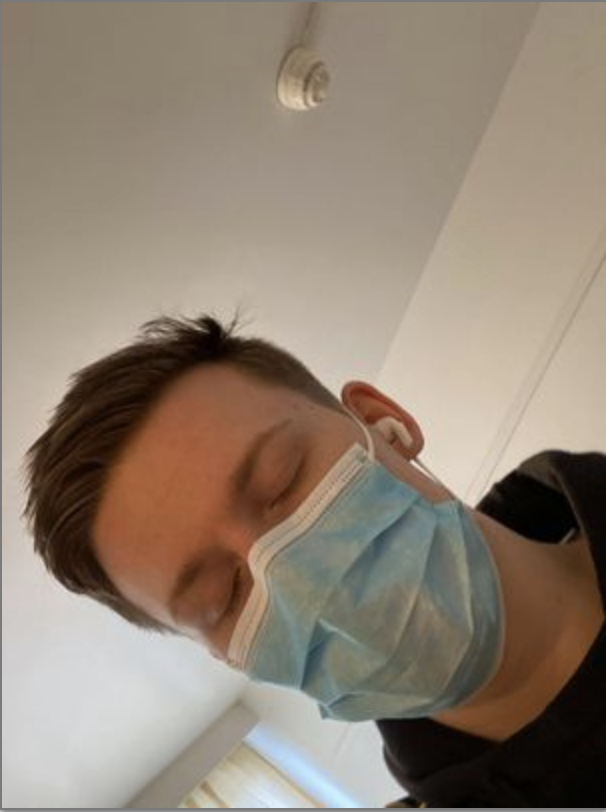
\includegraphics[scale = 0.295]{figures/0699.png}\hspace{0.4cm}}
    \caption{Different oblique angle camera shots.}
    \label{fig:tilt}
\end{figure}

As briefly mentioned in Section \ref{sec:delimit}, finding datasets that addressed and included facial images taken from oblique angles were hard to come by. The closest datasets we came by, only included facial images where the subjects had their heads tilted and not the camera which does not correspond to the same. Not only are the inclusion of the oblique angle facial image quite new, but our dataset furthermore mixed these images with face masks, which created an even more distinct dataset. 

\section{Second Subjective Experiment}
\label{sec:secondse}
A key part we wanted to achieve with the second subjective experiment was to make it as straight forward and understandable as possible. One should not have to be trained once more in order to understand and perform the subjective experiment. Therefore, we designed the second experiment as similar to our first one, and invited no new participants. The ground truth data was collected by running the experiment with six people who were the bachelor team, our supervisor and the product owner. The key elements of the experiment were: 
\begin{itemize}
    \item Randomizing the order of the images.
    \item Splitting it into two phases. 
    \item Using a category judgement.
\end{itemize}

The second experiment consisted of two phases. The first phase included the 250 undistorted images from NFC without splitting it into several connected experiment sessions as we did in our first experiment. Experience from our first experiment showed that the average duration to finish a session with 100 images was shorter than expected. We had initially planned for 100 images to be included in each session with an estimated duration time of around 15 minutes, but feedback from our participants showed that in most cases the experiments was finished in six to eight minutes. Based on those results, a subjective experiment with 250 images should not take longer than 25 minutes which is below the maximum limit of 30 minutes suggested by International Telecommunication Union \cite{methodologySubjective}. Although the experiment was 2.5 times larger than the sessions of the first experiment, only people directly involved with the project were expected to participate and so creating several sessions felt like unnecessary overhead. 

Even though our subjective experiment had new ways and aspects of testing the two FIQMs, we wanted to test them even further in phase two. The FIQMs ways of giving quality scores are based on how well you can see the face, explained in Chapter \ref{chap:FQA}, but the facial images' overall quality have an impact. We wanted to see how the two FIQMs would assess if we added distortions to the images. Based on this, we decided to extend our dataset by introducing different distortions to a number of images in our own dataset. Based on the results from the 250 images used in phase one of our second subjective experiment, we selected 10 images from each quality category and added distortions to them. This gave us 50 images to add each distortion on. We chose to add four different distortions, giving us 200 distorted images. From there, we conducted another subjective experiment, identical in design from phase one and with the same number of subjects which we referred to as the second phase of the subjective experiments. This subjective experiment consisted of the 200 distorted images, as well as the 50 original images selected from each quality category to be used as control images. In total, giving us 250 images to evaluate.

The type of distortions we added had to be reproducible, that way future research could add the same distortions and expect similar results. We added the following distortions: 
%
\begin{itemize}
    \item Compression with Telegram messaging application \footnote{\url{https://telegram.org/}}: The compression was done by messaging the images, resulting in change of the images' resolution and size.
    \item Compression with Adobe Photoshop (version 22.4): All images were compressed on compression level one.
    \item Noise with Adobe Photoshop: The images were added with noise of seven percent. 
    \item Blur with Adobe Photoshop: The images were added a blur level of two. 
\end{itemize}
%
Having two phases in the second subjective experiment, give us a considerable amount of data to test the two FIQMs on. Based on phase one and phase two, we can compare the subjective results from both phases and see how the subject's scores differ with distortions added to the images. Ideally, both the FIQMs-and subjective results should not differ in the two phases as long as the faces are visible in the images.


%The main purpose of the second subjective experiment was to label our dataset of 250 images and test the FIQMs, but we felt it lacked a clear difference from the first subjective experiment, and we figured including distorted images would make the difference. The second phase of the experiment was therefore made of 50 images, consisting of all subjects selected from the first dataset, but with distortions added to them. The point of the second phase was to see whether the participants would evaluate the face image quality of an undistorted and distorted image the same, and whether the FIQMs followed that statement. If the participants valued the images the same and the FIQMs did not, then the FIQMs would not provide the right scores, given that the scores are based on human assessment.  